\thispagestyle{empty}
\AddToShipoutPicture*{\put(0,0){%
\parbox[b][\paperheight]{\paperwidth}{%
\vfill
\centering
\refstepcounter{dummy}
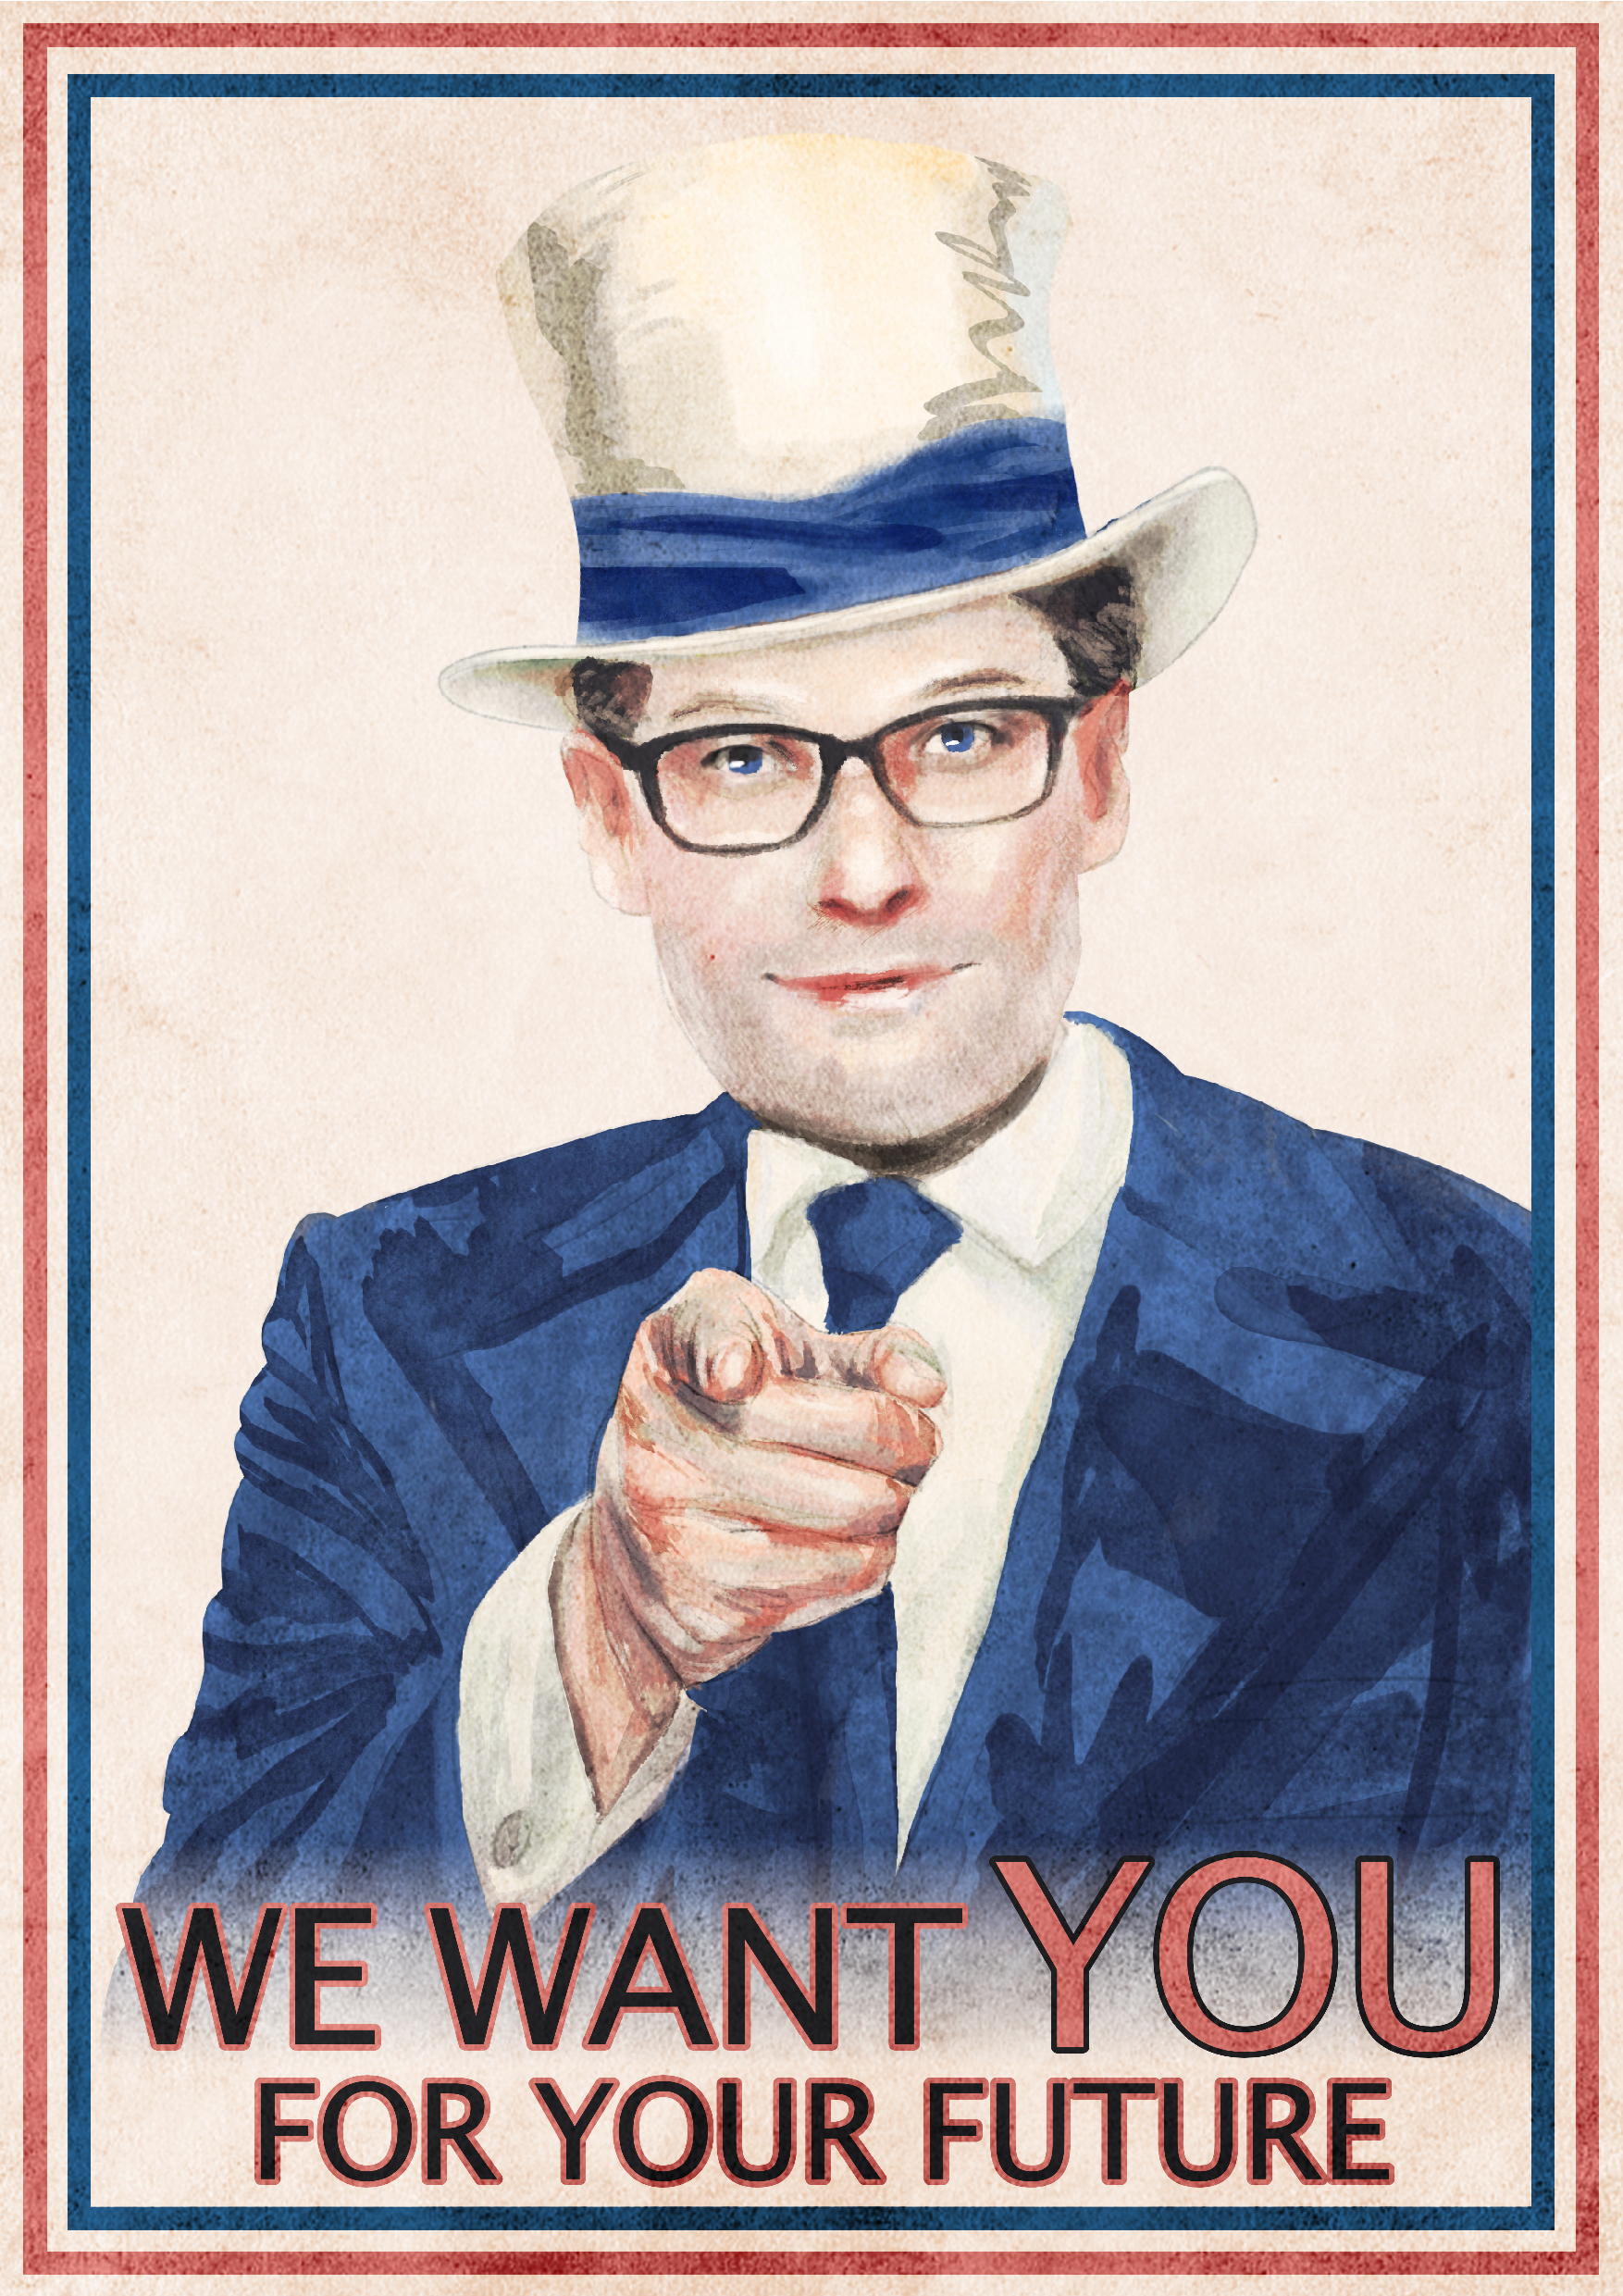
\includegraphics[width=\pagewidth]{img/we_want_you.pdf}%
\label{we_want_you}
\vfill
}}}
\
\pagebreak
\addchap{Grußwort}

\begin{wrapfigure}{l}{0.31\textwidth}
  \vspace{-12pt}
  \begin{centering}
    \includegraphics[width=0.3\textwidth]{img/sbalzarini.jpg}
  \end{centering}
  \caption*{\copyright MPI CPG}
  \vspace{-15pt}
\end{wrapfigure}

{\fontsize{10pt}{11}\selectfont
\selectlanguage{english}
Dear Students,

a wholehearted \enquote{Welcome} to the Faculty of Computer Science at TU Dresden! Congratulations for having decided to study computer science our university, as no other course of studies would nowadays open so many doors and provide you with so many opportunities like ours, and TU Dresden provides you with an excellent environment to pursue your goals in one of Germany’s most livable and affordable student cities.

We are a diverse, international, and interdisciplinary community of about 2400 students (every third from abroad), 220 scientists, 222 registered PhD students, 28 professors, 4 Honorary Professors, and two independent Group Leaders with the status of \enquote{TUD Young Investigator}. Together, we are one of the top computer science departments in Germany. We offer a selection of nine degree programs, including two international Master’s programs entirely taught in English. These curricula cover the entire breadth of our exciting discipline. And we are fortunate to do so under excellent conditions with state-of-the-art infrastructure. Our department is housed in a modern building offering generous teaching rooms and well-equipped labs. We have access to some of the best high-performance computing resources of Germany with machines hosted in a dedicated building just next door. Finally, our university's sports facilities are located just behind our building, and the student-run café \ascii{} in the Lobby of our building is a focal point of our social life.

Our building is proudly named after Prof. Andreas Pfitzmann, who was our chair of privacy and security until 2010. Andreas Pfitzmann's work was not only scientifically noted, but his social engagement had far-reaching consequences for the public opinion and the lawmaking in Germany. Andreas Pfitzmann is partly responsible for the fact that the German public has an internationally unparalleled level of awareness when it comes to topics of data protection, security, and privacy.  This is just one example of how computer science directly impacts and shapes many areas of our everyday lives. A young discipline, computer science is unique in its blend of being both a structural science, like mathematics and philosophy, and an engineering discipline. It has revolutionized the way we communicate with each other, the way we run organizations, manage industrial production, and do science in almost all disciplines. There is almost no area of science, technology, or society that would not be shaped by and depend on advancements in computer science. Computing is a universal language that reaches far beyond tech geekery and hobbyist programming. It is theory and algorithms that provide a rigorous mathematical understanding of "information processing". It is human-machine interaction and the human in the loop, linking our discipline to psychology and the arts. It is the information processing that happens in living cells and organisms by chemical signaling pathways and the neurons in our brains, linking to systems biology and medicine. It is machine learning and artificial intelligence that aim to produce \enquote{thinking machines}. It is data security and privacy with all its connections to the mathematics of cryptography, systems engineering, as well as societal and legal aspects. It is embedded systems, robotics, smart and autonomous systems with connections to electrical and mechanical engineering. Computer science is everywhere, and our faculty collaborates with pretty much every other department of TU Dresden, from medicine and environmental science, to mechanical and electrical engineering, to psychology and law in order to contribute toward solving humankind’s most challenging problems.

No wonder that computer science in Dresden is growing rapidly. Our faculty is set to enlarge with additional professorships, e.g., in the areas of data science and artificial intelligence. We have been extraordinarily successful in winning competitive national centers: We are hosting one of the nine National High-Performance Computing Centers (NHR) of Germany, one of the five Federal Centers for Machine Learning and AI, the ScaDS.AI Dresden/Leipzig, one of the four Centers for the next generation of mobile communication, 6G-Life, and one of only three DAAD Zuse Schools of Excellence in AI (SECAI). We are also a major partner in two DFG Clusters of Excellence (the Center for Tactile Internet, CeTI, and the Center for the Physics of Life, PoL), and we participate in the only Else-Kröner-Fresenius Center for Digital Health (EKFZ) in Germany. I am convinced you will benefit from the presence of these internationally visible top research and teaching centers with their unparalleled computational and academic infrastructure. 

Beyond our university, you will also benefit from the unique DRESDEN-concept alliance that the TU Dresden has founded with 32 non-university research institutions in our city. Dresden has been named as a city of Science in 2006 and has attracted an impressive number and concentration of research organizations. All major players are here with several institutes each: the Max Planck Society, the Helmholtz Association, the Fraunhofer Society, and the Leibniz Association, in addition to many research-active museums, hospitals, and cultural organizations. Under the common umbrella of DRESDEN-concept e.V., they greatly enrich your freedom of choice in finding exciting topics for your project modules, Bachelor's, Master's or Diplom thesis, or to stay on for a PhD after graduation. 

And if a PhD is not for you, then there are ample job opportunities in the IT industry in and around Dresden. The Saxon IT sector has been steadily growing by 5 to 7 \% per year since the German reunification. In Dresden alone, jobs for 600 to 800 computer science graduates are created each year. And this trend is set to further accelerate, as large multi-national corporations continue to move into our city. Some of them moved here specifically because of our degree programs and graduates,  that is because of you!

But first, you need to successfully master your studies. And that will be challenging. It is through challenges that we grow, as they say. So please consider the challenges you are undoubtedly going to meet in the coming semesters as such: challenges to grow on, not problems. A university is not a school. Many things are not predefined, there is a lot of freedom from designing your curriculum to deciding where to look for project topics. Welcome to the land of plenty! Benefit from the freedom and diversity of topics offered, but work systematically and diligently in order to not get lost in the multitude of possibilities. And if you do happen to get a bit lost, then please take advantage of the many counseling and mentoring offerings we provide for students. Work on developing your ability to learn independently and, most importantly, on your ability to judge yourself realistically. It is an easy trap to fool yourself into believing you have understood, and it is hard to know for sure when you actually did. Talking to others and actively and independently doing the exercises and homework is paramount to success. In a university, many problems are not "presented" to you, but you are expected to independently identify them. Likewise, you will be increasingly expected to be able to decide for yourself if one of your solutions is correct or not. Most people do not pass exams by simply sitting through lectures or reading a book. It is only through learning by doing in the exercises and tutorials that you achieve the ability to transfer knowledge to previously unseen problems. 

And for this journey of personal development, I wish you all the best of success! And of course fun. You will learn many fun things here and find many courses offered to you free of charge to satisfy your thirst for knowledge. Do not focus on the outcome, but enjoy the process! And do not hesitate to talk to us and become an active member of our community. Get engaged with the student association iFSR, find your network of friends and peers among the other students, ask senior students and tutors for advice, and do not hesitate to talk to your professors if you have questions or require help. We live a culture of open doors and wish to make your student experience here as rewarding and productive as possible. Probably the best example for this is the ESE, our welcome week for new students, which you are starting right now. The ESE is entirely student-organized, run by our student association, and financially supported by the faculty and by external sponsors. Big thanks to the iFSR and the sponsors! And now, dive in and enjoy the ride! Many exciting new things are awaiting you on your journey to becoming part of the global computer science community that shapes our future. 

   SHAPE YOUR FUTURE!

\textit{Ivo F. Sbalzarini,\\
Dean of the Faculty of Computer Science }
\selectlanguage{ngerman}
